
\chapter {\noun{Data Flows}}

Patients have access to the system by dedicated patient's application. 
Each patient is given unique, personal smart card that is being used for authentication.


\section{\textsc{Use Cases}}

The patient's application is a graphical interface to the patient's module. 
It includes six use cases that are available for the patient:
\begin{description}
\item[browse medicines] \hfill \\
The patient is able to browse all medicines available in the database. 
There is a leaflet attached to each medicine's description, that contains at least dosage and contraindications.
\item[browse pharmacies] \hfill \\
The patient is able to browse all pharmacies available in the database. 
Each pharmacy has its address and opening hours listed for patient's convenience.
\item[browse doctors] \hfill \\
The patient is able to browse all doctors available in the database. 
He can find phone number and office address for each doctor.
\item[browse prescription history] \hfill \\
The patient can browse all of his prescriptions, differentiated on active and already realized.
\item[transfer prescription] \hfill \\
If the patient cannot realize prescription, he is able to transfer his prescription buying rights to somebody else.
\item[cancel prescription transfer] \hfill \\
The patient can cancel transfer of prescription and realize it by himself or transfer it again.
\end{description}

\begin{figure}[h]
\fbox{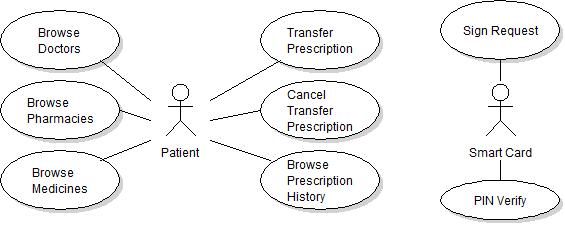
\includegraphics[scale=0.7]{patient/useCaseDiagram.jpg}}
\caption{Use cases}
\end{figure}

\section{\textsc{Smart card use cases}}
The smart card, introduced into the system for security reasons, includes two use cases.
\begin{description}
\item[sign message] \hfill \\
The smart card signs a message produced by patient's application. 
The signature would be used in calls to database procedures.
\item[verify PIN] \hfill \\
The smart card verifies PIN, that the patient has entered, in order to access any functionalities of the system.
\end{description}




\section{\textsc{Scenario: Prescriptions Transfer}}
\begin{enumerate}
\item To transfer a prescription a user has to enter correct PIN. 
\item The application establishes a connection with a database and retrieve the list of prescription available to transfer. 
\item The list contains only prescriptions which can be transferred by the patient. 
\item Then the patient is able to select prescription to transfer from the list and enter the new owner's ID. 
\item After the patient's confirms the transfer, the application creates and sends request to the database. 
\item If the signature under the request concatenated with nonce is valid and request contains required data, the database transfers the prescription to the new owner.
\end{enumerate}
\begin{figure}[h]
\centering
 \hspace*{-0.4in}
    \fbox{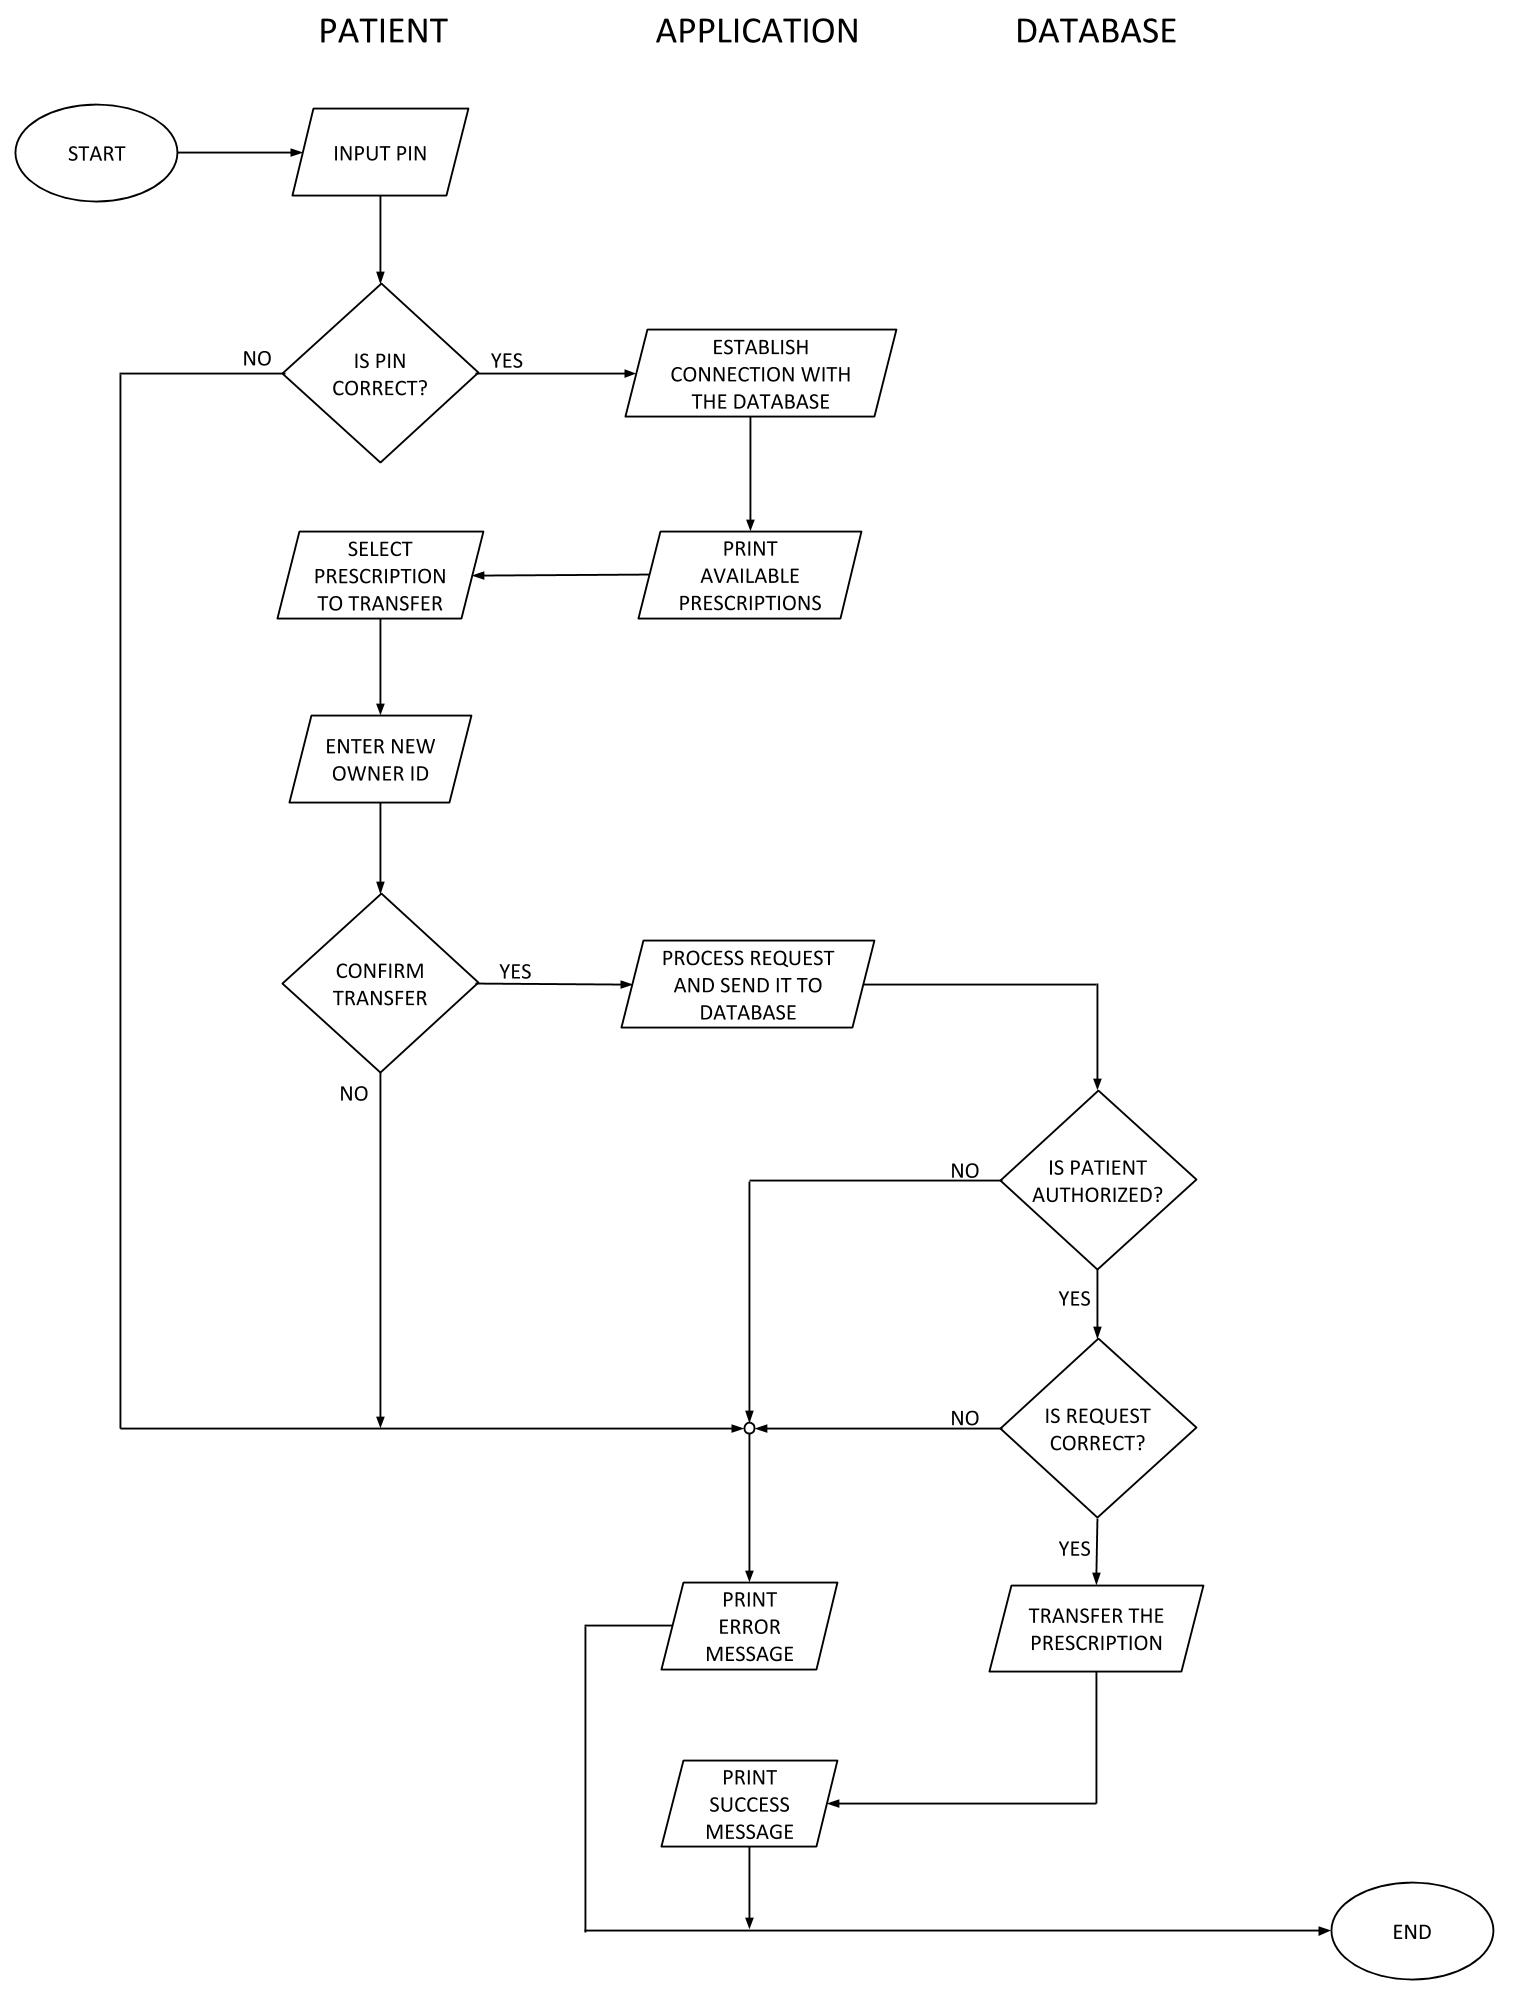
\includegraphics[width=0.78\textheight]{patient/transferPrescriptionFlowChart}}
\caption{Transfer prescription flow chart}
\end{figure}



\chapter {\noun{Functionalites of the Patient's Card}}


The patient's card implements functions described below.

\section{\textsc{Sign request}}

\begin{tabularx}{\textwidth}{ |p{2.5cm}|X| }
	\hline
	 &  \texttt{sign}\\
\hline	
argumets & 
\begin{itemize}
\item \texttt{message}
\end{itemize} \\
\hline
description & The patient's card signs doctor or pharmacist request.\\
\hline
action & 
The patient's card makes a signature under doctor or pharmacist message using its secret key.
\\
\hline
result &
\begin{itemize}
\item \texttt{signature}
\item \texttt{exit status}
\end{itemize}\\
\hline
\end{tabularx}

\section{\textsc{PIN verification}}

\begin{tabularx}{\textwidth}{ |p{2.5cm}|X| }
	\hline
	 &  \texttt{PIN\_verify}\\
\hline	
argumets & 
\begin{itemize}
\item \texttt{PIN}
\end{itemize} \\
\hline
description & 
The card verifies the PIN given by patient.\\
\hline
action & 
The patient's card verifies correctness of the PIN entered by the patient.\\
\hline
result &
\begin{itemize}
\item \texttt{exit status}
\end{itemize}\\
\hline
\end{tabularx}


\newpage

\chapter {\noun{Sequence diagrams}}

\FloatBarrier
\section{\textsc{Sequence diagram for connection initialization}}

\begin{figure}[!h]
\fbox{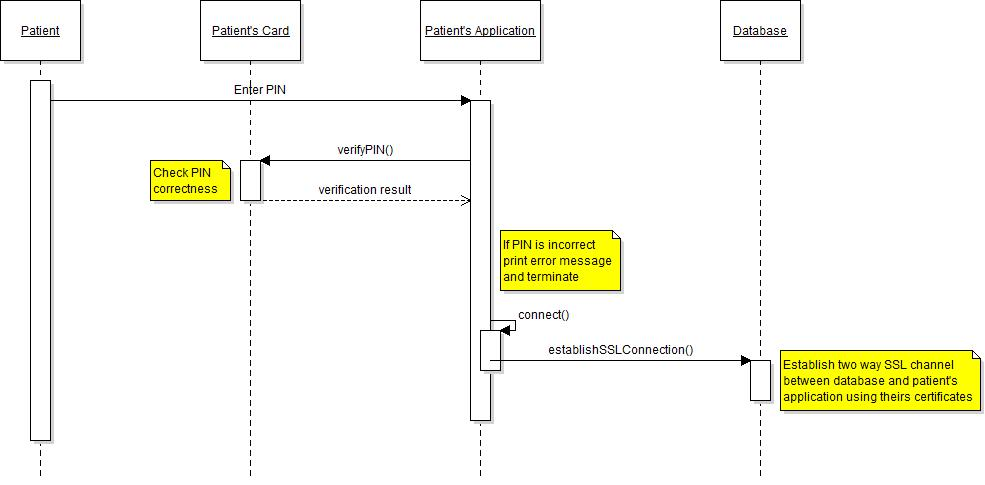
\includegraphics[width=0.93\linewidth]{patient/initializeConnectionSequenceDiagram}}
\caption{Connection initialization}	
\end{figure}
When the patient connects to the system, he needs to enter the PIN. 
Then, the PIN is verified by the Patient’s Card. 
If the verification fails, an error message is printed and the connection is terminated. 
Otherwise, the Patient’s Application establishes a two-way SSL channel with the database. 
From this point, the communication between the Patient’s Application and the database is done through SSL encrypted channel.

\FloatBarrier


\section{\textsc{Sequence diagram for transfer prescription functionality}}
\begin{figure}[!h]
\fbox{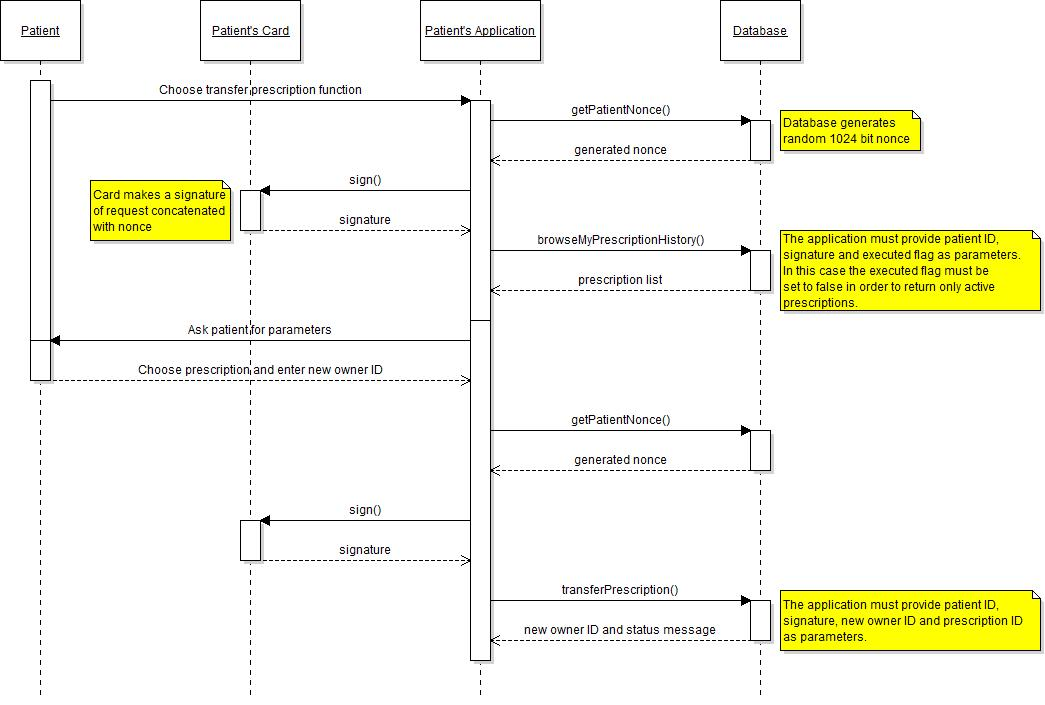
\includegraphics[width=0.93\linewidth]{patient/transferPrescriptionSequenceDiagram}}
\caption{Transfer prescription}
\end{figure}
This sequence is executed after establishing a secure connection with the database.\\

To transfer a prescription, the patient has to choose transfer prescription functionality in the Patient’s Application (PA). 
PA sends patient’s ID to the database and receives a random 1024 bit nonce. 
Afterwards, PA sends created browse prescriptions request to the Patient’s Card (PC) for signing. 
PA sends the signed request to the database (DB) and receives a list of available prescriptions. 
Then the patient chooses a prescription he wants to transfer from the list, and enters new owner’s ID.
Next, PA requests new nonce from DB and creates a valid transfer prescription request, which is signed by PC. 
The request with a signature is sent to DB afterwards. 
DB verifies both the request and the signature. If the verification was successful, DB transfers the prescription to the new owner and returns a status message and the ID of new owner.
\FloatBarrier

\section{\textsc{Sequence diagram for browse medicines functionality}}
\begin{figure}[!h]
\fbox{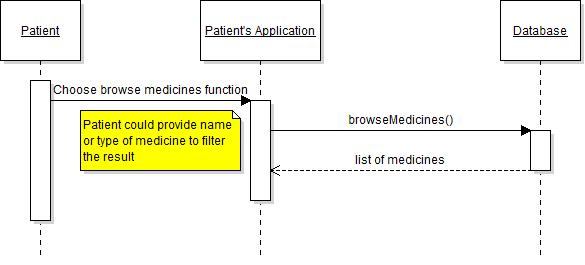
\includegraphics[width=0.93\linewidth]{patient/browseMedicinesSequenceDiagram}}
\caption{Browse medicines}
\end{figure}
To browse medicines, the patient needs to choose browse medicines functionality in the Patient’s Application. 
Then, the Patient’s Application prepares a request with parameters either default or provided by the patient. 
The request is sent to the database afterwards. 
The database returns a list of medicines which is displayed to the patient in the Patient’s Application.
\newpage


